\documentclass[tikz,border=6pt]{standalone}
\usetikzlibrary{arrows.meta,positioning}
\tikzset{
  op/.style  ={circle,draw,minimum size=7mm,inner sep=0pt},
  box/.style ={rectangle,draw,rounded corners=2pt,inner sep=2pt},
  >={Latex}
}
\begin{document}
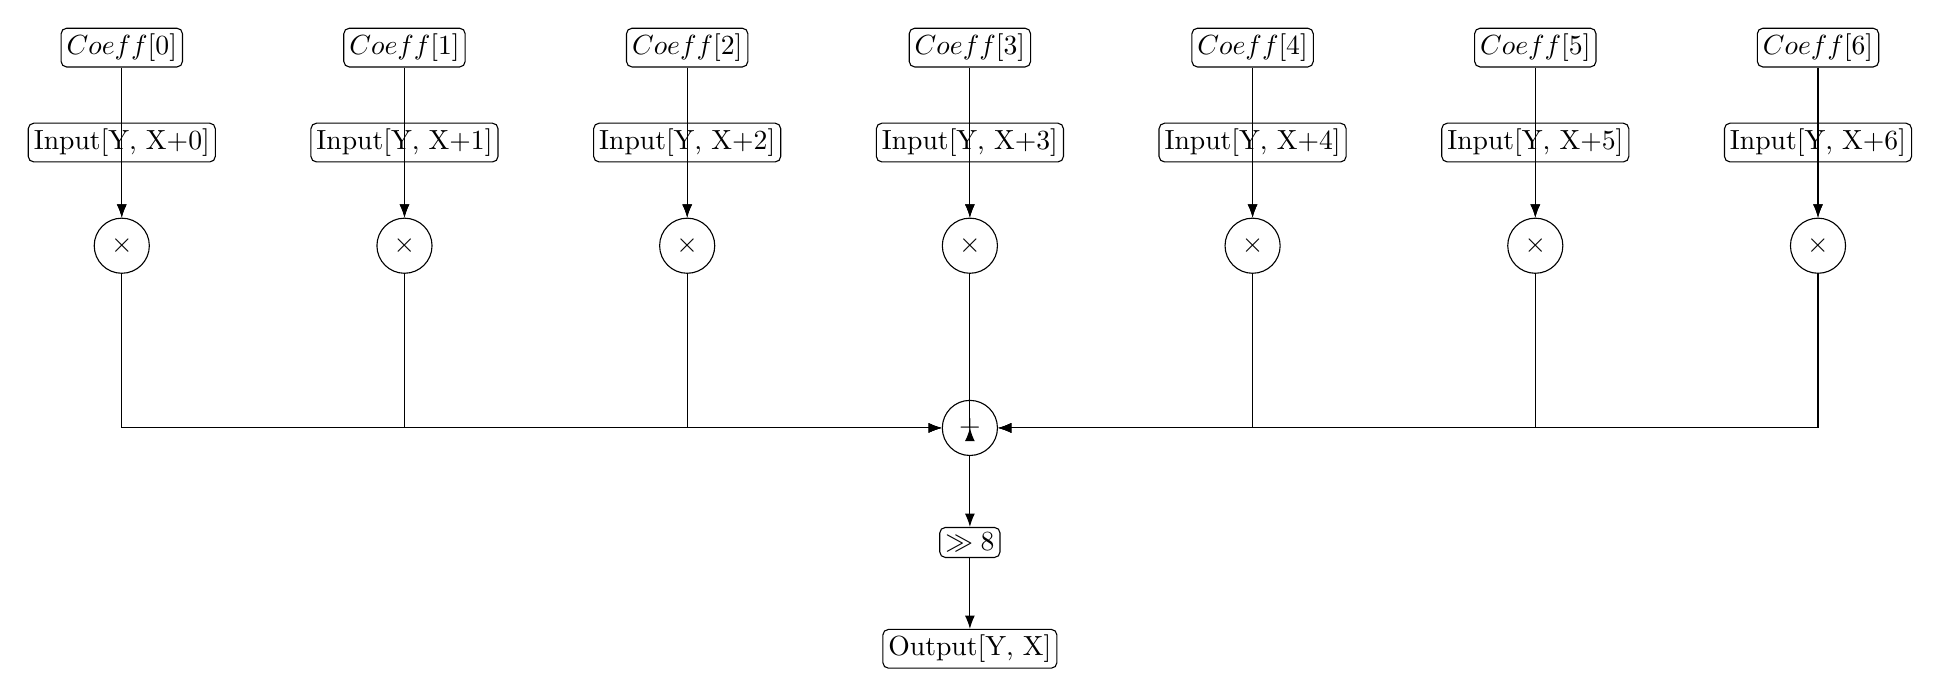
\begin{tikzpicture}[node distance=10mm and 10mm]

% -------- inputs (X+0..X+6) --------
\node[box] (i0) {Input[Y, X+0]};
\node[box, right=12mm of i0] (i1) {Input[Y, X+1]};
\node[box, right=12mm of i1] (i2) {Input[Y, X+2]};
\node[box, right=12mm of i2] (i3) {Input[Y, X+3]};
\node[box, right=12mm of i3] (i4) {Input[Y, X+4]};
\node[box, right=12mm of i4] (i5) {Input[Y, X+5]};
\node[box, right=12mm of i5] (i6) {Input[Y, X+6]};

% -------- coefficients --------
\node[box, above=7mm of i0] (c0) {$Coeff[0]$};
\node[box, above=7mm of i1] (c1) {$Coeff[1]$};
\node[box, above=7mm of i2] (c2) {$Coeff[2]$};
\node[box, above=7mm of i3] (c3) {$Coeff[3]$};
\node[box, above=7mm of i4] (c4) {$Coeff[4]$};
\node[box, above=7mm of i5] (c5) {$Coeff[5]$};
\node[box, above=7mm of i6] (c6) {$Coeff[6]$};

% -------- multipliers --------
\node[op, below=7mm of i0] (m0) {$\times$};
\node[op, below=7mm of i1] (m1) {$\times$};
\node[op, below=7mm of i2] (m2) {$\times$};
\node[op, below=7mm of i3] (m3) {$\times$};
\node[op, below=7mm of i4] (m4) {$\times$};
\node[op, below=7mm of i5] (m5) {$\times$};
\node[op, below=7mm of i6] (m6) {$\times$};

% wiring: inputs/coeffs -> multipliers
\foreach \a/\b in {i0/m0,i1/m1,i2/m2,i3/m3,i4/m4,i5/m5,i6/m6} \draw[->] (\a) -- (\b);
\foreach \a/\b in {c0/m0,c1/m1,c2/m2,c3/m3,c4/m4,c5/m5,c6/m6} \draw[->] (\a) -- (\b);

% -------- single adder collecting all 7 --------
\node[op, below=16mm of m3] (sum) {$+$};

\foreach \m in {m0,m1,m2,m3,m4,m5,m6} \draw[->] (\m) |- (sum);

% -------- shift and output --------
\node[box, below=9mm of sum] (sh) {$\gg 8$};
\node[box, below=9mm of sh] (out) {Output[Y, X]};
\draw[->] (sum) -- (sh);
\draw[->] (sh) -- (out);

\end{tikzpicture}
\end{document}
